\chapter{ روش پیشنهادی }
\section{مقدمه}

همان‌طور که در فصل‌ گذشته شرح داده شد، شناسایی چهره در محیط بدون محدودیت به صورت بی‌درنگ و با دقت بالا با چالش‌های بسیاری همراه است. همچنین دقت بالا و زمان پردازش پایین باهم در تضاد هستند. علاوه بر این‌ها، فرض ‌کمبود داده آموزشی نیز چالش بزرگی محسوب می‌شود. بنابراین در این فصل تلاش می‌کنیم تا روشی برای تشخیص بهتر و دقیق‌تر چهره توسط شبکه عصبی عمیق در تصاویر رنگی پیشنهاد دهیم. و مسئله کمبود داده‌های آموزشی را توسط معماری خاصی از شبکه های GAN برطرف نماییم.
\noindent
از آن‌جایی که ‌شبکه MobileNet معماری بسیار سبک تری نسبت به معماری های شناخته شده دیگر که در فصل ۲ معرفی شدند، دارد؛ بنابراین استخراج ویژگی‌ها از چهره و دسته بندی تصاویر چهره با دقت بالا برای این شبکه بسیار سخت و دشوار است. همچنین در مواردی شباهت چهره افراد به یکدیگر ‌کار را از آن‌چه هست سخت‌تر خواهد کرد. بنابراین ما روشی برای استخراج ویژگی از تصاویر چهره پیشنهاد کرده‌ایم که کمک می‌کند ویژگی‌های استخراج شده که متعلق به دو دسته متفاوت هستند، فاصله بیشتری از هم داشته باشند و در مقابل ویژگی های استخراج شده برای دو تصویر از چهره یک فرد یکسان، فاصله کمتری از هم داشته باشند؛ تا از این طریق بتوان به کاهش مشکلات ذکر شده کمک کرد. این روش شامل بخش‌های تولید چهره، یافتن چهره، آموزش شبکه عصبی پیچشی و ‌استخراج ویژگی می‌باشد.
\section{روش پیشنهادی}
دیاگرام
\begin{figure}[h]
\centering
  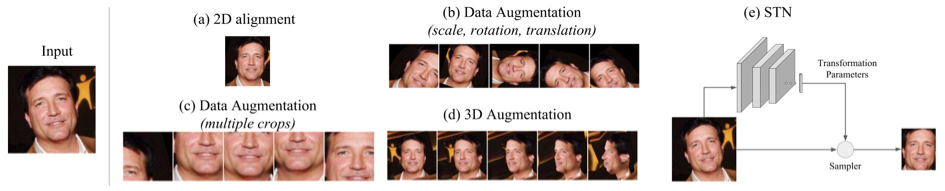
\includegraphics[scale=1]{image3-1}
  \caption{نمای کلی از روش پیشنهادی \cite{ref1}.}
  \label{image2-1}
\end{figure}

\subsection{پیش پردازش}
پیش‌پردازش شامل تصحیح گاما و اعمال فیلتر دوطرفه به منظور حذف نویز پس‌زمینه است. در ادامه به شرح مراحل پیش‌پردازش می‌پردازیم.
\subsubsection{یافتن چهره}
استفاده از رتینا
\subsubsection{تولید تصاویر آموزشی با \lr{GAN}}

در ادامه روند پیش‌پردازش، نوبت به تصحیح گاما می‌رسد. با این هدف که با استفاده از یک تبدیل غیرخطی روشنایی تصویر بهبود یابد. پس از پیش‌پردازش بالا، تصویر نسبت به قبل بهبود پیدا می‌کند اما پس از تکه تکه کردن تصویر جهت آموزش شبکه، تاریک بودن تصاویر مشهود است. برای حل این مشکل از گاما 0.8 استفاده می‌کنیم تا تصویر کمی روشن تر شود.
همچنین با تکه تکه کردن تصویر، نویزهایی در پس‌زمینه مشاهده می‌شود که ممکن است در فرآیند آموزش شبکه را دچار خطا کند. برای حذف این نویزها و در عین حال حفظ لبه‌ها در تصویر از فیلتر دوطرفه  استفاده می‌کنیم.
نتیجه اعمال این دو فرآیند را در تصویر زیر مشاهده می‌کنید. این نکته حائز اهمیت است که نتیجه حدف نویز در تکه‌های ایجاد شده از هر تصویر قابل مشاهده است.

استفاده از اف اس گن
\subsection{آموزش شبکه جهت استخراج ویژگی}
که پیش‌تر بیان شد به آموزش این شبکه می‌پردازیم. مشابه مرحله قبل از شبکه ResNet-50 برای آموزش استفاده می‌کنیم و ساختار آن مشابه آن چیزی است که در شکل ‏3 6 مشاهده می‌کنید. مجموعه داده خود را پس از پیش‌پردازش و افزایش‌ داده‌ها، آماده می‌کنیم. تعداد کل داده‌های آموزش برای این مرحله را به حدود 320000 رساندیم و آموزش را در 30 دوره انجام داده‌ایم.
\subsection{تابع ضرر}
یکی از چالش های اصلی در یادگیری ویژگی ها با استفاده از شبکه های عصبی عمیق پیوسته \lr{(DCNN)} برای شناسایی چهره در مقیاس بزرگ، طراحی تابع ضرر مناسب است که قدرت تفکیک را افزایش می‌دهد. هدف ما کم کردن فاصله بین ویژگی‌های عمیق و مراکز کلاس‌های آن‌ها در فضای اقلیدسی برای دستیابی به فشردگی درون کلاسی بیشتر می‌باشد. ما یک تابع ضرر برای افزایش زاویه ای حاشیه برای دستیابی به ویژگی های بسیار متمایز برای تشخیص چهره پیشنهاد می‌کنیم که عملکرد بهتر برخوردار است و می توان آن را به راحتی با هزینه های محاسباتی ناچیز پیاده سازی کرد.
\noindent
برای آموزش شبکه های عصبی عمیق پیوسته برای تشخیص چهره، دو رویکرد اصلی وجود دارد. روش اول دسته بندی را آموزش می دهند که می تواند هویت های مختلف را در مجموعه آموزش از هم جدا کند، مانند با استفاده از طبقه بندی \lr{softmax}، و رویکرد دوم که مستقیماً یک تعبیه را یاد می گیرند، مانند \lr{triplet loss}. بر اساس داده های آموزش در مقیاس بزرگ و معماری \lr{DCNN}، هر دو روش می توانند عملکرد بسیار خوبی در تشخیص چهره داشته باشند. با این حال، هم رویکرد \lr{softmax} و هم رویکرد \lr{triplet loss} اشکالاتی دارد.
\noindent
برای :
\begin{enumerate}
\item
	اندازه ماتریس تبدیل W به طور خطی با افزایش تعداد دسته ها \lr{(n)} افزایش می یابد.‌
\item 
ویژگیهای آموخته شده برای مسئله‌های طبقه بندی با مجموعه بسته قابل تفکیک هستند اما به اندازه کافی برای مسئله تشخیص چهره که یک مسئله باز می‌باشد، مناسب نیستند. 
\end{enumerate}
\noindent
برای \lr{triplet loss}:
\begin{enumerate}
\item
 برای مجموعه داده های مقیاس بزرگ، رشد شدید در تعداد ترکیب‌های تعداد تصاویر سه گانه وجود دارد که منجر به افزایش قابل توجه تعداد مراحل تکرار می‌شود.
\item 
 استخراج مجموعه تصاویر سه گانه یک مسئله دشوار برای آموزش موثر می‌باشد. 
\end{enumerate}
\noindent
ما برای افزایش بیشتر قدرت تمایز مدل تشخیص چهره و ایجاد ثبات در روند آموزش، تابع ضرر مبتنی بر توابع مثلثاتی را پیشنهاد می‌کنیم. همانطور که در شکل 2 نشان داده شده است، حاصل ضرب نقطه ای مقادیر موجود در ویژگی های استخراج شده و آخرین لایه کاملاً متصل، برابر با ضرب کسینوسی آن‌ها پس از نرمال سازی می باشد‌، ما از تابع مثلثاتی کسینوسی برای محاسبه زاویه بین ویژگی فعلی و وزن هدف استفاده می‌کنیم. سپس یک حاشیه زاویه ای به زاویه هدف اضافه می‌کنیم‌، در انتها با استفاده از تابع کسینوس دوباره مقادیر را به فضای خطی برمی‌گردانیم. مراحل بعدی دقیقاً مانند \lr{softmax} هستند.
مزایای این روش پیشنهادی را می‌توان به شرح زیر خلاصه کرد:
\begin{itemize}
 \item
در مجموعه داده های تصویر و فیلم در مقیاس بزرگ ، به عملکرد مناسبی دست می یابد.
 \item
فقط به چندین خط کد نیاز دارد و اجرای آن در چارچوب های یادگیری عمیق مبتنی بر  Pytorch و Tensorflow آسان است. برای داشتن عملکرد پایدار نیازی به ترکیب با سایر توابع ضرر ندارد و به راحتی همگرا می‌شود.
 \item
هنگام آموزش فقط پیچیدگی محاسباتی ناچیز را اضافه می کند. پردازنده های گرافیکی کنونی می توانند به راحتی از هزاران دسته مختلف برای آموزش پشتیبانی کنند و مدل به راحتی می تواند هویت های بیشتری را پشتیبانی کند.
\end{itemize} 
\noindent


رابطه ریاضی \lr{softmax} معروف ترین تابع ضرر طبقه بندی که به طور گسترده استفاده می شود، به شرح زیر است:
 \begin{equation}\label{eq3-2}
L= - \frac{1}{N} \sum_{i=1}^{N} log \frac{e^{{W_{y_i}^T} x_i + b_{y_i}}}{\sum_{j=1}^{n} e^{{W_j^T} x_i + b_j}} 
\end{equation}
\noindent
که در آن \lr{xi} نشان دهنده ویژگی عمیق نمونه \lr{i} ازدسته \lr{y} است. تعداد ابعاد ویژگی استخراج شده را 512 در نظر گرفتیم. \lr{Wj} ستون \lr{j}  ام از وزن \lr{W} می‌باشد و \lr{bj} بایاس است. مقدار \lr{N}اندازه دسته و \lr{n} تعداد دسته‌ها است. این تابع مستقیما ویژگی استخراج شده را برای اعمال شباهت بالاتر برای نمونه های درون کلاس و فاصله بیشتر برای نمونه های بین کلاسی بهینه نمی‌کند، که منجر به ایجاد مشکل در عملکرد آن برای تشخیص چهره عمیق تحت تغییرات ظاهری بزرگ درون کلاس می شود (به عنوان مثال تغییرات زاویه چهره و تقییرات سنی).

\noindent
ما رابطه فوق را مبنای محاسبات قرار دادیم و تغییرات جزیی به آن اضافه کردیم. برای سادگی مقدار بایاس را صفر در نظر گرفتیم. سپس حاصل ضرب مقادیر موجود در ویژگی های استخراج شده و آخرین لایه کامل
متصل را به صورت
$W_j^T x_i = ||W_j|| ||x_i|| cos(θ_j)$
تبدیل می کنیم، که \lr{θj} زاویه بین وزن \lr{Wj} و ویژگی \lr{xi} است. نرمال سازی ویژگی‌ها و وزن‌ها باعث می‌شود که خروجی فقط به زاویه بین ویژگی و وزن بستگی داشته باشد. به کمک نرمال سازی مقادیر وزن $||W_j||$ را برابر ۱ در نظر می‌گیریم. همچنین ویژگی استخراج شده $||x_i||$ را نرمال کرده و نام آن را \lr{s} در نظر می‌گیریم. ‌‌‌بنابرین ویژگی‌های استخراج شده در یک ابر کره با شعاع s توزیع می‌شوند. برای افزایش حاشیه بین \lr{xi} و \lr{Wj} یک مقدار \lr{m}اضافه می‌کنیم تا به طور همزمان فشرده سازی درون کلاسی و اختلاف بین کلاسی را افزایش دهیم.
 \begin{equation}\label{eq3-2}
L = - \frac{1}{N} \sum_{i=1}^{N} log \frac{e^{s(cos(\theta_{y_i}+m))}}{e^{s(cos(\theta_{y_i}+m))} + \sum_{j=1}^{n} e^{s(cos(\theta_j))}}
\end{equation}
\noindent
همانطور که در شکل 3 نشان داده شده است، \lr{softmax} ویژگی‌های تقریباً قابل تفکیکی ایجاد می‌کند اما در مرزهای تصمیم گیری ابهام قابل توجهی به وجود می‌آید، در حالی که تابع ضرر ما می تواند فاصله بیشتری را بین دسته‌های نزدیک اعمال کند.
\begin{figure}[h]
\centering
  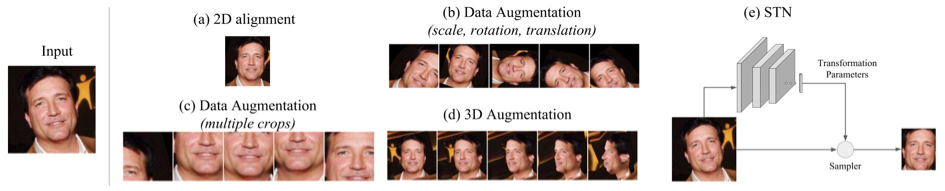
\includegraphics[scale=1]{image3-1}
  \caption{رویکردهای مختلف هم ترازی چهره \cite{ref1}.}
  \label{image2-1}
\end{figure}

 \begin{figure}[h]
\centering
  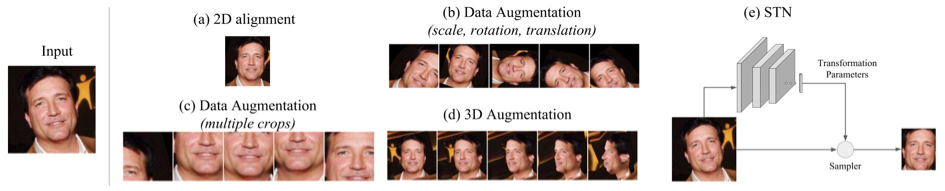
\includegraphics[scale=1]{image3-1}
  \caption{رویکردهای مختلف هم ترازی چهره \cite{ref1}.}
  \label{image2-1}
\end{figure}

\subsubsection{مدل پيشنهادي پايه}

\subsubsection{دسته‌بندی}
مسير استخراج ويژگي از پنج لايه كانولوشن، چهار لايه خطي اصلاح شده ۱ و نرمال ساز دستهاي۲ ، چهار لايه ديكانولوشن۳ و شش ماژول se-voxres ، كه در ادامه توضيح داده خواهد شد، استفاده شده است. تصوير ورودي I به بخش استخراج ويژگي داده ميشود و مدل در اين مسير به طور خودكار يك سلسله مراتب ويژگي را از تصاوير ورودي آموزش خواهد ديد و در نهايت اين ويژگيهاي استخراج شده از لايههاي مختلف با يكديگر
تركيب شده و به عنوان ورودي تقسيمبند مورد استفاده قرار ميگيرد ]۱۴[ .
• لايه كانولوشن
سه لايه كانولوشن همراه با گام دو، اندازه حجم ورودي را با ضريبي از دو كاهش ميدهد. سايز پنجره فيلترها 3 × 3 ميباشد. دليل انتخاب سايز كوچك پنجره فيلترها كاهش پيچيدگي محاسباتي و همچنين عملكرد خوب آنها در استخراج ويژگي ميباشد. چگونگي عملكرد يك لايه كانولوشن از رابطه ۲.۳ بدست
ميآيد.

در مرحله آزمون به منظور بررسی یک تصویر فوندوس، پس از پیش‌پردازش تصویر را مطابق با ورودی شبکه اول تکه تکه می‌کنیم و جهت استخراج میکروآنوریسم‌های کاندید به آن شبکه می‌دهیم. پس از استخراج پیکسل‌های کاندید، به مرکز این پیکسل‌ها تکه‌ای به اندازه ورودی شبکه دوم می‌زنیم تا این شبکه ویژگی‌های لازم را استخراج کند. همچنین ویژگی‌های دست‌ساز را هم از این کاندیدها استخراج کرده و جهت دسته‌بندی به ماشین بردار پشتیبان می‌دهیم. در شکل ‏3 11 یک تصویر فوندوس را مشاهده می‌کنید که در تصویر سمت چپ مکان اصلی میکروآنوریسم‌ها را نشان می‌دهد و در سمت راست نتیجه الگوریتم به منظور شناسایی میکروآنوریسم‌ها را می‌بینید.

\subsubsection{آموزش‌}
در ابتداي روند آموزش، لازم است پارامترهاي مدل مقدار دهي اوليه شوند و انتخاب پارامترهاي اوليه ميتواند تأثير زيادي در مدل آموزش يافته داشته باشد. در اين پژوهش به منظور مقدار دهي اوليه پارامترها از تابع توزيع يكنواخت استفاده شده است. از ديگر چالشهاي اساسي براي روشهاي بهينه سازي مبتني بر گراديان، انتخاب ميزان نرخ يادگيري مناسب است. روشهاي كلاسيك گراديان تصادفي از نرخ يادگيري ثابت يا كاهشي استفاده ميكنند، كه براي همه پارامترهاي مدل يكسان است. با اين حال، مشتقات جزئي پارامترهاي لايههاي
EFTL =
(1−Tverskyc)1/γ (۱۲.۳)
۷۵
مختلف ميتوانند از نظر مقدار متفاوت باشند، كه ميتواند به نرخ يادگيري مختلفي نياز داشته باشد. با اين حال، مشتقات جزئي پارامترهاي لايههاي مختلف ميتوانند از نظر مقدار تفاوت قابل توجهي داشته باشند، كه ميتواند به نرخ يادگيري مختلفي نياز داشته باشد. در سالهاي اخير، تمايل به توسعه روشهايي براي انتخاب خودكار نرخ يادگيري مستقل افزايش يافته است. اكثر روشها )به عنوان مثال، RMSprop، [۴۸]AdaDelta، [۴۷]AdaGrad]۴۹[ و Adam]۵۰[( آمارهاي مختلف مشتقات جزئي را در چندين تكرار جمع آوري ميكنند و از اين اطلاعات براي تعيين ميزان يادگيري سازگار براي هر پارامتر استفاده ميكنند. اين امر به ويژه براي آموزش شبكههاي عميق بسيار مهم است، جايي كه نرخ يادگيري مطلوب اغلب براي هر لايه بسيار متفاوت است. در اين پژوهش در آزمايشات انجام شده از همه روشهاي نام برده استفاده شد ولي روش Adam عملكرد بهتري ارائه داده است.


شکل ‏3 4- قبل و بعد از اعمال تصحیح گاما و فیلتر دوطرفه در یک تکه بیمار مبتنی بر ناحیه
استخراج تکه
برای آموزش شبکه نیاز داریم تا تصاویر فوندوس پیش‌پردازش شده را تکه تکه کنیم. زیرا میکروآنوریسم بسیار ریز بوده و تشخیص آن در یک تصویر کلی برای شبکه کاری بسیار دشوار است. از آن‌جایی که در تصویر برچسب‌زده شده، نقاط میکروآنوریسم دقیقا مشخص شده‌اند می‌توانیم با تکه تکه کردن تصویر و مشخص کردن مناطق میکروآنوریسم در هر تکه، آموزش را برای شبکه ساده‌تر کنیم. زیرا به جای دادن کل تصویر به شبکه، تکه‌های ایجاد شده را جهت آموزش به شبکه می‌دهیم.
برچسب‌زدن به تکه‌ها
در بسیاری از مقالات در این زمینه و زمینه‌های مشابه برای برچسب زدن به این روش عمل کرده‌اند که اگر پیکسل مرکز تکه، یک پیکسل از ناحیه میکروآنوریسم باشد، به کل تکه برچسب بیمار یا یک تخصیص می‌یابد و اگر پیکسل مرکز ناحیه‌ای از میکروآنوریسم نباشد برچسب سالم یا صفر برای تکه در نظر گرفته می‌شود. این روش برچسب زدن یک مشکل عمده دارد. اگر شبکه با این روش برچسب‌زدن آموزش یابد، شبکه یاد می‌گیرید که با توجه به نواحی مشاهده شده، برای پیکسل مرکز تصمیم بگیرد که سالم است یا حاوی میکروآنوریسم. بنابراین برای آزمون یک تصویر فوندوس کلی باید به ازای تمام پیکسل‌های یک تصویر و به مرکز آن‌ها تکه انتخاب کرد و به شبکه جهت ارزیابی داد. با این وجود حتی اگر دقت شبکه خیلی بالا هم باشد، به علت زیاد بودن تعداد تکه‌های انتخاب شده، مثبت‌های کاذب و منفی‌های کاذب بسیار زیادی خواهیم داشت.
بنابراین در این روش ما برچسب‌زدن را به دو روش انجام خواهیم داد. در ابتدا نواحی کاندید در تصویر فوندوس را با استفاده از آموزش به طریق توجه به وجود میکروآنوریسم در تکه پیدا خواهیم کرد و پس از آن در نواحی کاندید به روش توجه به پیکسل مرکز به نواحی اصلی و دقیق میکروآنوریسم دست پیدا خواهیم کرد.
برچسب ‌زدن با توجه به وجود میکروآنوریسم در تکه (مبتنی بر ناحیه)
همان‌طور که گفته شد این روش برچسب زدن به منظور انتخاب کردن نواحی کاندید انجام شده است. به این صورت که در ابتدا سعی می‌کنیم نواحی دارای میکروآنوریسم را مشخص کنیم و پس از آن در نواحی کاندید جستجو کنیم و پیکسل‌های دقیق را پیدا کنیم. برای پیدا کردن نواحی کاندید باید روش برچسب زدن را با توجه به میکروآنوریسم در تکه انجام دهیم. به این صورت که اگر میکروآنوریسم در داخل تکه قرار داشت برچسب بیمار و اگر وجود نداشت برچسب سالم را به آن تکه می‌دهیم. برخی از پژوهش‌ها مانند آنچه توسط چادزیک  و همکاران [34] بیان شده است از این روش استفاده کرده‌اند. اما یک مشکل در این روش وجود دارد. اگر میکروآنوریسم فقط در یک یا چند پیسکل حاشیه تکه وجود داشته باشد، تشخیص آن نه تنها برای شبکه بلکه برای انسان نیز سخت خواهد بود.
برای رفع این مشکل تدبیری در این کار در نظر گرفته شده است. در این روش به تکه برچسب بیمار را می‌دهیم اگر و فقط اگر عارضه میکروآنوریسم به طور کامل درون پچ قرار گرفته باشد. همچنین ایجاد یک فاصله چند پیکسلی از اطراف تکه نیز می‌تواند به تشخیص آسان‌تر میکروآنوریسم کمک کند. به این صورت که اگر به طور مثال اندازه تکه 101 پیکسل باشد، تکه‌ای برچسب بیمار را دریافت می‌کند که میکروآنوریسم به طور کامل در داخل تکه 80 در 80 پیکسلی داخل تکه اصلی قرار گرفته باشد.
برچسب زدن با توجه به پیکسل مرکز (مبتنی بر پیکسل مرکز)
پس از استخراج نواحی کاندید، بر آنیم که از بین نواحی محتمل، نواحی واقعی میکروآنوریسم را به کمک روش پیکسلی مشخص کنیم. بنابراین نیازمند روش دیگری برای برچسب زدن تکه‌ها هستم. برای این منظور به این صورت عمل می‌کنیم که اگر پیکسل مرکز تکه یک پیکسل میکروآنوریسم بود به کل تکه برچسب بیمار و در غیر این صورت برچسب سالم را می‌دهیم. در مقاله [31] افتخاری و همکاران از همین روش برچسب زدن استفاده شده است. به صورتی که در گام اول به علت زیاد بودن تکه‌های سالم، این تکه‌ها به صورت کاملا تصادفی انتخاب شده‌اند.
اما در این کار ما روشی دیگر را برای انتخاب تکه در نظر گرفته‌ایم. برای انتخاب تکه‌های سالم دو مرحله در نظر گرفته‌ایم.
در ابتدا به صورت تصادفی تکه‌های کاملا سالم را انتخاب می‌کنیم. یعنی تکه‌هایی که اصلا اثری از میکروآنوریسم در آن‌ها وجود ندارد. این کار باعث می‌شود که یادگیری شبکه برای تشخیص تکه سالم و بیمار ساده‌تر شود.
حال در مرحله دوم تکه‌های نیمه سالم را انتخاب ‌می‌کنیم. این تکه‌ها،‌ تکه‌هایی هستند که میکروآوریسم در آن‌ها وجود دارد اما پیکسل مرکز را شامل نمی‌شود. دلیل نام‌گذاری نیز همین موضوع است که تکه نیمه‌سالم است، زیرا طبق روش برچسب‌زنی پیکسلی، مرکز شامل میکروآنوریسم نمی‌باشد و از طرفی اثرهایی از میکروآنوریسم در تکه دیده می‌شود.
توجه به این نکته در انتخاب تکه الزامی است که در انتخاب تکه نیمه سالم باید دقت کرد که میکروآنوریسم زیاد به پیکسل مرکز نزدیک نشود تا کار یادگیری برای شبکه سخت نشود. انتخاب یک حاشیه امن برای پیکسل مرکز به اندازه بین 10 تا 15 پیکسل مناسب است که میکروآنوریسم از این فاصله به پیکسل مرکز نزدیک‌تر نشود.
دلیل انتخاب تکه‌های نیمه سالم این است که شبکه فقط به وجود یا عدم وجود میکروآنوریسم توجه نکند. بلکه وجود میکروآنورسیم در مرکز تکه را در دستور کار قرار دهد. بنابراین وجود این تکه‌ها در داده‌های آموزشی باعث می‌شود که شبکه مرز را بهتر یاد بگیرد. در شکل ‏3 5 نمونه‌ای از تکه بیمار، نیمه سالم و سالم مشاهده می‌کنید.

 
شکل ‏3 5- انواع تکه‌ها در روش برچسب زدن با توجه به پیکسل مرکز
انتخاب نوع شبکه و اندازه مناسب تکه
حال نوبت آن است که اندازه مناسب برای تکه‌ها و نوع مناسب شبکه برای مسئله را به دست آوریم. اگر اندازه تکه بسیار کوچک باشد، منطقه میکروآنوریسم ناحیه بزرگ‌تری نسبت به اندازه تکه را در بر می‌گیرد اما از آن‌جایی که نواحی وسیعی از اطراف قابل مشاهده نیست ممکن است این میکروآنوریسم با یک قسمت از یک رگ اشتباه گرفته شود. در مقابل، اگر اندازه تکه بسیار بزرگ در نظر گرفته شود، اندازه میکروآنوریسم نسبت به اندازه تکه بسیار کوچک خواهد بود و کار را برای تشخیص شبکه سخت می‌کند و امکان ایجاد منفی کاذب، یعنی ناحیه‌ای که میکروآنوریسم وجود دارد اما به اشتباه سالم تشخیص داده‌ایم، افزایش می‌یابد.
ما آزمایش‌های مختلف با اندازه‌های مختلف تکه برای انواع مختلف شبکه انجام داده‌ایم. این آزمایش به این صورت است که با اندازه‌های مختلف 101 در 101، 81 در 81، 51 در 51 و 33 در 33 پیکسل تصاویر فوندوس را تکه تکه کردیم و به دو روشی که عنوان شد عمل برچسب‌ زدن را انجام دادیم و با شبکه‌های به‌روز و متداول از جمله Xception، VGG16، VGG19، ResNet-50، ResNet-101، ResNet-152، InceptionV3 و IncetionResNetV2 به کمک یادگیری انتقال و همچنین شبکه‌های سفارشی مندرج در برخی مقاله‌ها آموزش دادیم. آزمون را بر روی حدود 20000 تکه ارزیابی که به نسبت مساوی تکه بیمار و سالم تقسیم شده‌اند انجام داده‌ایم. نتایج سه شبکه برتر از نظر معیار‌های ارزیابی دقت، حساسیت و ویژگی در جدول ‏3 1، جدول ‏3 2 و جدول ‏3 3 مشاهده می‌کنید. 


آزمایش‌هایی با اندازه‌های بزرگ‌تر از 101 نیز انجام شد که به علت ضعیف بودن نتایج در جدول‌ها درج نشده‌اند. از نتایج جدول‌ها متوجه می‌شویم که بهترین اندازه تکه برای روش برچسب زنی مبتنی بر ناحیه، 33 پیکسل و برای روش برچسب زنی مبتنی بر پیکسل مرکز، 101 پیکسل است و همچنین برای استفاده از هر دو روش، بهترین معماری شبکه معماری ResNet-50 است.
روش پیشنهادی
پس از بیان مقدمات لازم، نوبت به شرح روش می‌رسد. روش پیشنهادی ما مبتنی بر توجه به پیسکل‌های کاندید است که از دو مرحله تشکیل شده است. در مرحله اول با استفاده از روش مبتنی بر ناحیه، پیکسل‌های کاندید و محتمل میکروآنوریسم را در یک تصویر فوندوس شناسایی می‌کنیم. این کار بر اساس روش مبتنی بر ناحیه انجام خواهد شد. در مرحله دوم از بین نواحی کاندید، به روش مبتنی بر پیکسل مرکز آزمون گرفته می‌شود که نواحی دقیق میکروآنوریسم شناسایی شوند.
استخراج پیکسل‌های کاندید
برای این منظور در ابتدا نیازمند آموزش شبکه عصبی پیچشی مبتنی بر ناحیه هستیم. پس مجموعه داده آموزشی خود را آماده می‌کنیم. در تمام تصاویر فوندوس که از قبل پیش‌پردازش شده‌اند اطراف نواحی میکروآنوریسم تکه‌هایی با اندازه 33 در 33 پیکسل استخراج می‌کنیم مطابق با روش برچسب زدن مبتنی بر ناحیه برچسب بیمار را به آن‌ها می‌دهیم. همچنین هر تصویر با به صورت تصادفی تحت تاثیر چرخش 90 درجه، چرخش 180 درجه، چرخش 270 درجه، برگرداندن عمودی و برگرداندن عمودی قرار می‌دهیم تا مجموعه داده افزایش بیابد. در مجموع تعداد کل داده‌های بیمار به حدود 230000 تکه رسید.
حال، به همین تعداد تکه بیمار و با همان روش برچسب زدن مبتنی بر ناحیه به طور تصادفی تکه سالم استخراج می‌کنیم. سعی شده است که تکه‌های سالم بیشتر از نواحی نزدیک به تکه‌های بیمار انتخاب شوند. در این صورت به علت شباهت نسبی پس‌زمینه بین تکه سالم و تکه بیمار مجاور، تمرکز شبکه به یادگیری میکروآنوریسم بیشتر جلب خواهد شد.
در انتها، مجموعه داده ما شامل حدود 460000 تکه سالم و بیمار آماده برای آموزش شبکه ResNet-50 می‌شود. در آموزش شبکه لایه‌های استخراج بردار ویژگی و دسته‌بندی نهایی به صورت سفارشی مناسب با مسئله خودمان طراحی کرده‌ایم و برای آموزش لایه‌های ابتدایی که تقریبا برای تمام مسائل یکسان هستند را ثابت در نظر می‌گیریم. زیرا این لایه‌ها کار تشخیص خطوط، زوایا و سایر ویژگی‌های یکسان در تمام مجموعه داده‌ها را انجام می‌دهند و نیاز به آموزش مجدد نیست و در انتها لایه‌های سفارشی خود را اضافه می‌کنیم و آموزش می‌دهیم که به این کار یادگیری انتقال می‌گویند. شکل ‏3 6 نمایی از شبکه عصبی مورد استفاده و لایه‌های سفارشی در انتهای ساختار را نشان می‌دهد. 

 
شکل ‏3 6- یادگیری انتقال در آموزش شبکه عصبی پیچشی مبتنی بر ناحیه

پس از آموزش شبکه در 30 دوره بر روی داده‌های آموزشی، می‌توان از این شبکه برای استخراج پیکسل‌های کاندید استفاده کرد.
روند کار برای استخراج پیکسل‌های کاندید به این صورت است که ابتدا بر روی تصویر اصلی با یک تعداد گام کوتاه 5 پیکسل شروع به حرکت می‌کنیم و تکه‌های 33 در 33 پیکسل استخراج می‌کنیم. تکه‌های استخراج شده را جهت ارزیابی به شبکه می‌دهیم و احتمال بیمار بودن را به تک تک پیکسل‌های داخل آن تکه تخصیص می‌دهیم.
با این روش به جز پیکسل‌های مرزی، سایر پیکسل‌ها در چندین تکه حضور دارند. بنابراین دو ماتریس به اندازه طول و عرض تصویر فوندوس تشکیل می‌دهیم. یکی از این ماتریس‌ها مشخص می‌کند که هر پیکسل در چند تکه‌ حضور داشته است (Count). و دیگری مجموع احتمالات هر پیکسل که در تکه‌های ارزیابی حضور داشته است را در خود نگهداری می‌کند (SumOfProbs). در نتیجه میانگین احتمال بیمار بودن هر پیکسل از طریق رابطه (3-1) به دست می‌آید.

(3-1)	Probs[R][C] = SumOfProbs[R][C]  / Count[R][C]
در مقاله‌ها احتمال به دست آمده از شبکه را مستقیما به تک‌تک پیکسل‌های آن تکه نسبت می‌دهند. ما در این کار به روشی دیگر عمل کرده‌ایم.
باید این نکته را مدنظر قرار داد که هر چه به پیکسل‌های حاشیه تکه نزدیک می‌شویم، تاثیر آن پیکسل در نتیجه احتمال به دست آمده کمتر می‌شود. به صورتی که می‌توان گفت پیکسل‌های مرزی احتمال صفر دارند. بنابراین احتمال به دست آمده را به طور یکسان به تمام پیکسل‌ها نسبت نمی‌دهیم. بلکه قبل از این کار از توزیع نرمال استفاده می‌کنیم. این توزیع نرمال ماتریسی دو بعدی هم اندازه با تکه یعنی 33 در 33 پیکسل است و با نام Weights مشخص شده است که در شکل ‏3 7 مشاهده می‌کنید. پس برای هر پیکسل، وزن معادل آن مشخص شده است. احتمال به دست آمده از شبکه را در وزن مربوطه هر پیکسل ضرب می‌کنیم تا احتمال بیمار بودن آن پیکسل در تکه به دست آید. احتمال حاصل را به درایه جدول SumOfProbs متناظر با آن پیکسل اضافه می‌کنیم و به این صورت این جدول تکمیل خواهد شد.

 
شکل ‏3 7- ماتریس وزن‌ها معادل توزیع نرمال مربوط به تکه‌های 33 در 33 پیکسل

روش معمول مقالات که به صورت ضمنی برای پر کردن جدول Count استفاده می‌کنند به این صورت است که پس از بررسی هر تکه، برای هر پیکسلی که در تکه حضور دارد، یک واحد به درایه متناظر آن پیکسل در جدول Count اضافه می‌کنند. اما در این کار به جای یک واحد، وزن آن پیکسل در تکه مورد بررسی را به درایه متناظر در جدول Count اضافه می‌کنیم. به عنوان مثال اگر در یک تکه پیکسلی در سطر 16 و ستون 15 باشد به درایه Count آن پیکسل 0.9375 واحد اضافه می‌کنیم.
به طور خلاصه برای پیکسلی که در سطر R و ستون C از تصویر اصلی قرار دارد و در داخل تکه 33 در 33 در سطر r و ستون c قرار دارد مجموع احتمالات و تعداد (تعداد وزن‌دار) از رابطه (3-2) و (3-3) به دست می‌آید.

(3-2)	SumOfProbs[R][C] = SumOfProbs[R][C] + CNNProb × Weights[r][c]
(3-3)	Count[R][C] = Count[R][C] + Weight[r][c]

پس از استخراج تمام تکه‌ها و دادن آن‌ها به شبکه اول و محاسبه احتمال میانگین برای هرپیکسل، نوبت به مشخص کردن پیکسل‌های کاندید می‌رسد. پیکسل‌هایی که دارای احتمال بالای 0.7 هستند را به عنوان کاندید در نظر می‌گیریم. 
در نگاه اول شاید عدد 0.7 زیاد به نظر آید. زیرا بهتر است که شبکه اول مثبت‌های کاذب بیشتر داشته باشد تا شبکه دوم میکروآنوریسم‌ها را از مثبت‌های کاذب تشخیص دهد. اما با انجام آزمایش‌های مختلف این عدد انتخاب شده است و مثبت‌های کاذب به اندازه کافی تولید می‌کند. چون شبکه به صورتی آموزش دیده است که برای میکروآنوریسم‌های تشخیصی خود احتمال بالای 0.9 در نظر می‌گیرد. پس عدد 0.7 شاهد مثبت‌های کاذب زیادی خواهد بود.
	شناسایی پیکسل‌های میکروآنوریسم از میان پیکسل‌های کاندید
حال نوبت آن است که از میان پیکسل‌های کاندید انتخاب شده از مرحله قبل، پیکسل‌های میکروآنوریسم را تشخیص دهیم. برای این منظور به مرکز پیکسل‌های کاندید تکه‌های 101 در 101 پیکسل تشکیل می‌دهیم و این تکه را به شبکه عصبی آموزش دیده مبتنی بر پیکسل مرکز می‌دهیم تا احتمال بیمار بودن پیکسل مرکز را برای ما مشخص کند.
مطابق آنچه فزودن ویژگی‌های دست‌ساز به بردار ویژگی شبکه
پس از آموزش شبکه، می‌توان از این شبکه برای دسته‌بندی استفاده کرد. اما به منظور بهبود ویژگی‌های استخراج شده از این شبکه، تعدادی ویژگی دست‌ساز مهمی را که در [28] ذکر شده است به بردار ویژگی شبکه اضافه می‌کنیم. زیرا کیفیت ویژگی‌های استخراج شده به طور مستقیم بر روی دقت تشخیص میکروآنوریسم اثر می‌گذارد. ویژگی‌ها را از کانال سبز و آبی به طور مساوی استخراج ‌می‌کنیم تا مکمل یکدیگر باشند. این ویژگی‌ها که در مقاله مذکور بیان شده‌اند به شرح زیر هستند:
	ویژگی‌های مبتنی بر نمایه برش تقاطعی  
نمایه مجموعه‌ای از مقادیر پیکسل‌ها است که از نقاط با فاصله منظم در راستای یک بخش به ‌دست می‌آید و برش تقاطعی مقادیر پیکسل‌ها در امتداد یک بخش، نمایه برش تقاطعی نامیده‌ می‌شود. همان‌طور که در شکل ‏3 8 مشاهده می‌شود معمولا نمایه برش تقاطعی میکروآنوریسم‌ها در هر جهت توزیع گاوسی مشخص و مشابهی را نشان می‌دهد و در مقابل توزیع شدت نمایه‌های مختلف کاندید‌های اشتباه مثل عروق خونی در جهت‌های مختلف متفاوت هستند.. با توجه به این مشخصه مجموعه‌ای از ویژگی‌های آماری از نمایه برش تقاطعی در جهت‌های مختلف قابل استخراج است که برای تشخیص میکروآنوریسم بسیار مفید هستند.
زاویه بین خطوط برش تقاطعی، شش درجه در نظر گرفته شده است که بیانگر 30 خط برش تقاطعی است و طول خطوط 31 در نظر گرفته شده است. هر نمایه برش تقاطعی به صورت یک بردار با نام pi در نظر گرفته شده است و میانگین نمایه برش تقاطعی با یک بردار با نام pm مشخص می‌شود که هر درایه آن میانگین شدت نمایه مربوطه را نشان می‌دهد. علاوه بر این، یک منحنی گاوسی بر روی pm برازش می‌کنیم که با g نمایش می‌دهیم. حال ویژگی‌های زیر را استخراج می‌کنیم:

الف) اختلاف بین میانگین و کمینه بردار میانگین نمایه برش تقاطعی (pm):
ب) میانگین ضرایب همبستگی بین تمام نمایه‌های برش تقاطعی pi و میانگین نمایه برش تقاطعی (pm).
	ج) انحراف معیار ضرایب همبستگی بین تمام نمایه‌های برش تقاطعی pi و میانگین نمایه برش تقاطعی (pm).
	د) میانگین اختلاف‌های عادی‌ شده  بین تمام نمایه‌های برش تقاطعی pi و میانگین نمایه برش تقاطعی (pm). 	هر اختلاف عادی شده به صورت رابطه (3-5) محاسبه می‌شود:

که N طول هر نمایه را نشان می‌دهد.
	ه) انحراف معیار از تمام اختلاف‌های عادی شده


 
شکل ‏3 8- نمونه‌ای از خطوط برش تقاطعی و نمایه‌های برش تقاطعی از کاندید‌های میکروآنوریسم بازچاپ از [55]. a میکروآنوریسم صحیح و b و c کاندید‌های اشتباه هستند.

	ویژگی‌های مبتنی بر تبدیل برش تقاطعی
در مقاله [28] برای تقویت ویژگی‌های کاندیدهای میکروآنوریسم، یک تصویر محلی تبدیل برش تقاطعی محلی (LCT)  تولید شده است و ما از این ویژگی‌ها نیز برای تقویت بردار ویژگی خود استفاده می‌کنیم.
برای هر پیکسل کاندید یک تصویر محلی 31 در 31 پیکسلی به مرکز آن پیکسل استخراج می‌کنیم و 30 نمایه برش تقاطعی استخراج می‌کنیم و این بردارها را در یک ماتریس قرار می‌دهیم که هر ستون این ماتریس بیانگر یک نمایه برش تقاطعی است. به این ترتیب یک تصویر 31 در 30 پیکسلی تبدیل برش تقاطعی تولید شده است. شکل ‏3 9 یک نمونه LCT از میکروآنوریسم واقعی و دو کاندید اشتباه را نشان می‌دهد. همان‌طور که در شکل می‌بینید، در تصویر اصلی پیش‌پردازش شده تفاوت بین میکروآنوریسم واقعی و کاندیدهای اشتباه از ویژگی‌های بافت‌نگار گرادیان‌های جهت‌دار  HOG)) حاصل نمی‌شود. درحالی که تصویر LCT به طور قابل توجهی تفاوت ویژگی‌های HOG را بین میکروآنوریسم‌های واقعی و اشتباه را افزایش می‌دهد. زیرا نسبت میکروآنوریسم در تصویر LCT حدود چهار برابر میزان میکروآنوریسم در تصویر اصلی آن است و در این تصویر در میان میکروآنوریسم‌های واقعی گرادیان افقی به صورت قابل ملاحظه‌ای افزایش یافته است و تغییرات گرادیان عمودی حساس‌تر شده است.
 
شکل ‏3 9- تجسم ویژگی HOG  از تصویر پیش‌پردازش شده در مقابل تصویر تبدیل برش تقاطعی بازچاپ از [55]. a میکروآنوریسم صحیح و b و c کاندیدهای اشتباه هستند.

با در نظر گرفتن کل تصویر محلی به عنوان سلول ویژگی‌های زیر را استخراج می‌کنیم.
الف) prehog: استخراج ویژگی‌های HOG از تصویر پیش‌پردازش شده محلی. ابتدا اندازه و جهت گرادیان هر پیکسل را محاسبه می‌کنیم. سپس آمار بافت‌نگار HOG تصویر را در 9 جهت محاسبه می‌کنیم. بنابراین ویژگی‌های HOG را در یک بردار نه بعدی استخراج کرده‌ایم.
ب) transhog: همان ویژگی‌های HOG بر روی تصویر LCT
	آموزش SVM برای دسته‌بندی کاندیدها
تا این‌جا توانسته‌ایم سه نوع ویژگی را استخراج کنیم. نوع اول، ویژگی‌هایی است که از طریق آموزش شبکه عصبی پیچشی به دست می‌آید. نوع دوم ویژگی‌های مبتنی بر نمایه برش تقاطعی و نوع سوم ویژگی‌های مبتنی تبدیل برش تقاطعی است. حال از تمام ویژگی‌های منتخب مطابق شکل ‏3 10 برای آموزش یک ماشین بردار پشتیبان (SVM) استفاده می‌کنیم و در مرحله آزمون، ویژگی‌های عنوان شده را استخراج کرده و به کمک یک ماشین بردار پشتیبان سالم و یا بیمار (دارای میکروآنوریسم) بودن آن تکه را مشخص می‌کنیم. 


 
شکل ‏3 10- دسته‌بندی ویژگی‌های استخراج شده از تکه به کمک ماشین بردار پشتیبان

\section{نتیجه گیری}

 
شکل ‏3 11- مکان میکروآنوریسم‌های اصلی و میکروآنوریسم‌های شناسایی شده توسط روش پیشنهادی در یک تصویر فوندوس